\documentclass[a4paper]{article}

\usepackage[english]{babel}
\usepackage[utf8]{inputenc}
\usepackage{amsmath}
\usepackage{graphicx}
\usepackage[colorinlistoftodos]{todonotes}
\usepackage[export]{adjustbox}[2011/08/13]
\usepackage{float}

\title{Behaviour Dynamics in Social Networks - Assignment 4}

\author{Maria Hotoiu, Federico Tavella}

\date{\today}

\begin{document}
\maketitle

\begin{abstract}
Learn to use parameter tuning tools to find the best values for a set of missing parameter values in a model.
\end{abstract}

\section{Part 1}

\begin{figure}[!htpb]
\center
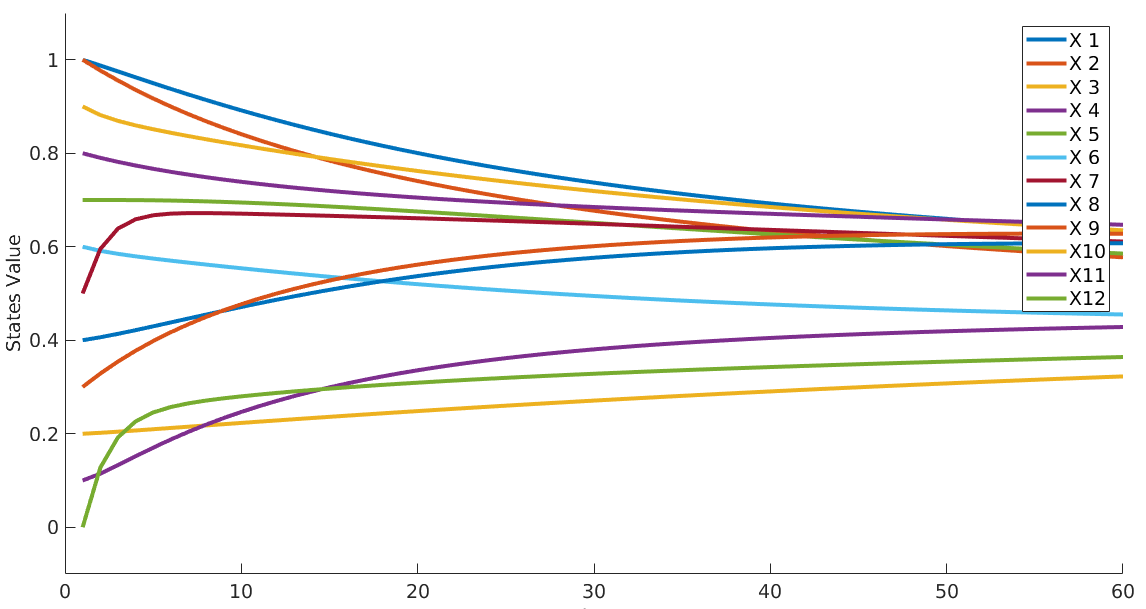
\includegraphics[width=1.2\textwidth]{res/img/part1}
\caption{Results from the simulation}
\label{fig:part1}
\end{figure}

\section{Part 2}


\begin{table}[!htpb]
\centering
\begin{adjustbox}{width=1.2\textwidth,center=\textwidth}
\begin{tabular}{c|c|c|c|c|c|c|c}
\textbf{$\eta_{L}$} & \textbf{K(t = 2)} & \textbf{L(t = 2)} & \textbf{$|$K-L(t = 2)$|$} & \textbf{K(t = 13)} & \textbf{L(t = 13)} & \textbf{$|$K-L(t = 13)$|$} & \textbf{Sum of differences} \\ \hline
0                   & 0.1146            & 0                 & 0.1146                    & 0.2221             & 0                  & 0.2221                     & 0.3367                      \\
0.05                & 0.1146            & 0.0127            & 0.1019                    & 0.2395             & 0.1232             & 0.1162                     & 0.2181                      \\
0.10                & 0.1146            & 0.0255            & 0.0892                    & 0.2517             & 0.1949             & 0.0568                     & 0.1460                      \\
0.15                & 0.1146            & 0.0382            & 0.0765                    & 0.2603             & 0.2359             & 0.0243                     & 0.1008                      \\
0.20                & 0.1146            & 0.0509            & 0.0637                    & 0.2664             & 0.2592             & 0.0072                     & 0.0709                      \\
0.25                & 0.1146            & 0.0636            & 0.0510                    & 0.2708             & 0.2724             & 0.0016                     & 0.0526                      \\
0.30                & 0.1146            & 0.0764            & 0.0383                    & 0.2739             & 0.2799             & 0.0060                     & 0.0443                      \\
0.35                & 0.1146            & 0.0891            & 0.0256                    & 0.2763             & 0.2844             & 0.0081                     & 0.0337                      \\
0.40                & 0.1146            & 0.1018            & 0.0128                    & 0.2781             & 0.2873             & 0.0092                     & 0.0220                      \\
0.45                & 0.1146            & 0.1145            & 0.0001                    & 0.2795             & 0.2892             & 0.0097                     & 0.0098                      \\
0.50                & 0.1146            & 0.1273            & 0.0126                    & 0.2806             & 0.2906             & 0.0100                     & 0.0226                     
\end{tabular}
\end{adjustbox}
\caption{Exhaustive search for different values of $\eta_{L}$}
\label{tab:exaustive_search}
\end{table}

\section{Part 3}

\begin{table}[H]
\centering
\begin{adjustbox}{width=0.4\textwidth,center=\textwidth}
\begin{tabular}{c|c|c}
\textbf{$\eta_{L}$} & \textbf{SSR} & Error\\ \hline
                                                                                                                 
                                   
0 & 0.9593 & 0.0816  \\                                       
0.05 & 0.0222 &  0.0124  \\
0.1  & 0.0463  & 0.0179 \\
0.15  &  0.1618 & 0.0335  \\  
0.2  & 0.2621   & 0.0427\\
0.25 & 0.3402 &  0.0486\\
0.3 & 0.4010 &  0.0528  \\
0.35 & 0.4491  &  0.0558  \\ 
0.4  & 0.4881 & 0.0582 \\
0.45  & 0.5202 &  0.0601\\
0.5 &  0.5472 & 0.0616 
\end{tabular}
\end{adjustbox}
\caption{Exhaustive search for different values of $\eta_{L}$}
\label{tab:exaustive_searchSSR}
\end{table}
The best value for $\eta_{L}$ is $\eta_{L}$=0.05.

\begin{figure}[H]
\center
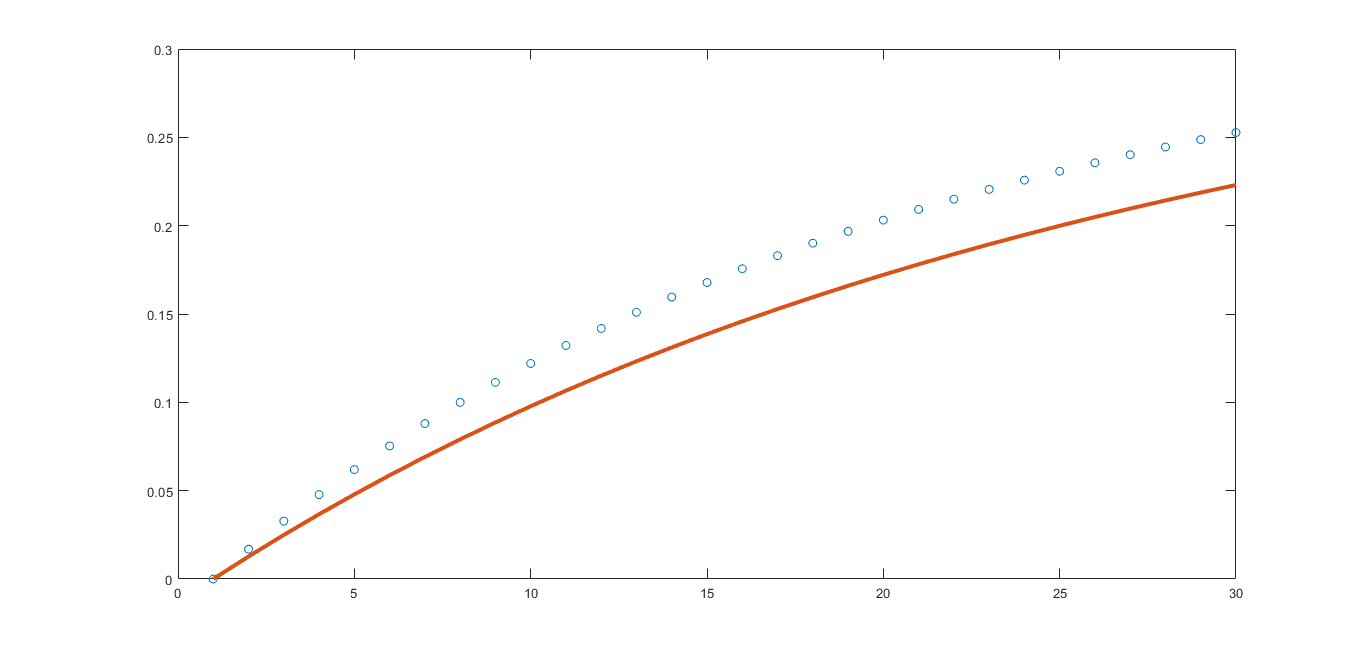
\includegraphics[width=1.3\textwidth]{res/img/plotdiff}
\caption{Simulated values for  $\eta_{L}$=0.05 (line) vs empirical values (dots)}
\label{fig:part3}
\end{figure}

\section{Part 4}


\begin{table}[H]
\centering
\begin{tabular}{c|c}
\textbf{$\eta_{i}$} & \textbf{value} \\ \hline
                            
$\eta_{1}$ & 0.21 \\                                       
$\eta_{2}$ & 0.11 \\ 
$\eta_{3}$ & 0.06 \\ 
$\eta_{4}$ & 0.12 \\ 
$\eta_{5}$ & 0.1 \\ 
$\eta_{6}$ & 0.04 \\ 
$\eta_{7}$ & 0.15 \\ 
$\eta_{8}$ & 0.21 \\ 
$\eta_{9}$ & 0.14 \\ 
$\eta_{10}$ & 0.03 \\ 
$\eta_{11}$ & 0.2 \\ 
$\eta_{12}$ & 0.162 \\ 

\end{tabular}
\caption{Exhaustive search for different values of $\eta$}
\label{tab:exaustive_searchSSR}
\end{table}

If we want to use exhaustive search with grain size of 0.01, we should check $101^{12}$ sets of values.

\end{document}
